%% ==================
\section{Application}
\label{sec:BIQueries}
%% ==================

Rationale and evaluation approach with respect to addressing the business requirements noted in Section~\ref{sec:Introduction}, i.e. how have you used the case studies / BI Queries to address and demonstrate the attainment of your business requirements.


%% ===============================
\subsection{BI Query 1: Which genre has the most active engagement on Twitter}
\label{sec:BIOne}
%% ===============================

For this query, the contributing sources of data are: \ldots

The general findings are that \ldots as illustrated in \figurename~\ref{fig:query1}.

\begin{figure}[ht]
\centering
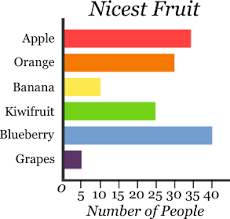
\includegraphics[width=.5\textwidth]{./figures/query1}
\caption{Results for BI Query 1}
\label{fig:query1}
\end{figure}

%% ===============================
\subsection{BI Query 2: \ldots}
\label{sec:BITwo}
%% ===============================

For this query, the contributing sources of data are: \ldots

The general findings are that \ldots as illustrated in \figurename~\ref{fig:query1}.

\begin{figure}[ht]
\centering
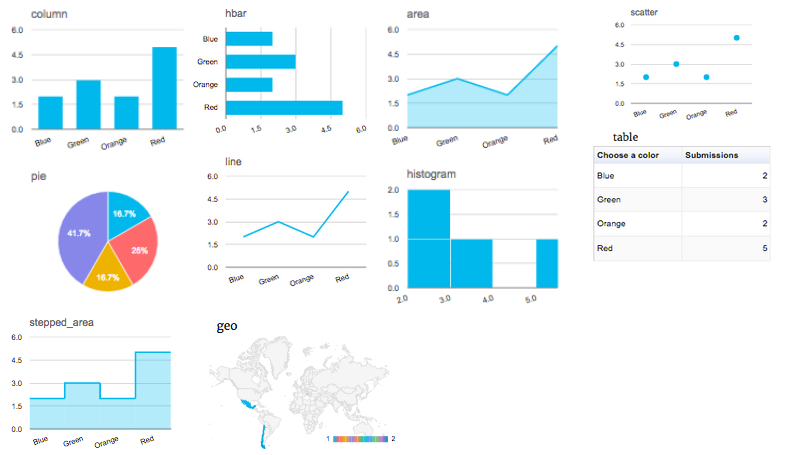
\includegraphics[width=.75\textwidth]{./figures/dashboard}
\caption{Results for BI Query 2}
\label{fig:query2}
\end{figure}

%% ===============================
\subsection{BI Query 3: \ldots}
\label{sec:BIThree}
%% ===============================

For this query, the contributing sources of data are: \ldots

The general findings are that \ldots as illustrated in \figurename~\ref{fig:query1}.

\begin{figure}[ht]
\centering
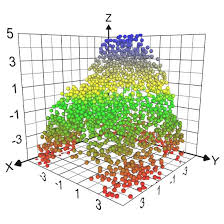
\includegraphics[width=.5\textwidth]{./figures/query3}
\caption{Results for BI Query 3}
\label{fig:query3}
\end{figure}

%% ===============================
\subsection{Discussion}
\label{sec:discussion}
%% ===============================

A detailed discussion / summarisation of the findings from the 3 queries. Note that this discussion will have a lot more detail than the discussion in the following section (Conclusion). You should relate your main findings to the literature that you reviewed in Section~\ref{sec:rw}, i.e. those with a similar topic to your data warehousing project (but which are not necessarily data warehousing projects), and compare and contrast your findings with theirs. 